% Project Specifications
%\clearpage%if the chapter heading starts close to bottom of the page, force a line break and remove the vertical vspace
\vspace{21.5pt}
\chapter{Project Specifications/Background}

Metropolia computer labs are including new courses based on raspberry pi pico. boards, running micropython.

These boards need resetting between classes to the specified software needed.

It is possible to setup the software in such a state that it will not communicate with a PC due to boot time runing scripts.

It should be possible to recover these boards to a bootable state without fully wiping them.

Ideally, this should be done without any loss of data.

It is also desirable to be able to quickly erase all data without wiping the software.

It would be convenient to be able touse one pico to do this to another, due to ready availibility, and also as a demonstration of what can be done with one.

Should auto detect correct type of pi board for ease of use, pico and pico w need different firmwares.

Should work standalone and not require PC.

\section{Overview of Raspberry Pi Pico}

\begin{figure}[ht]
	\centering
	\AltText{Stock photo of Raspberry Pi Pico}{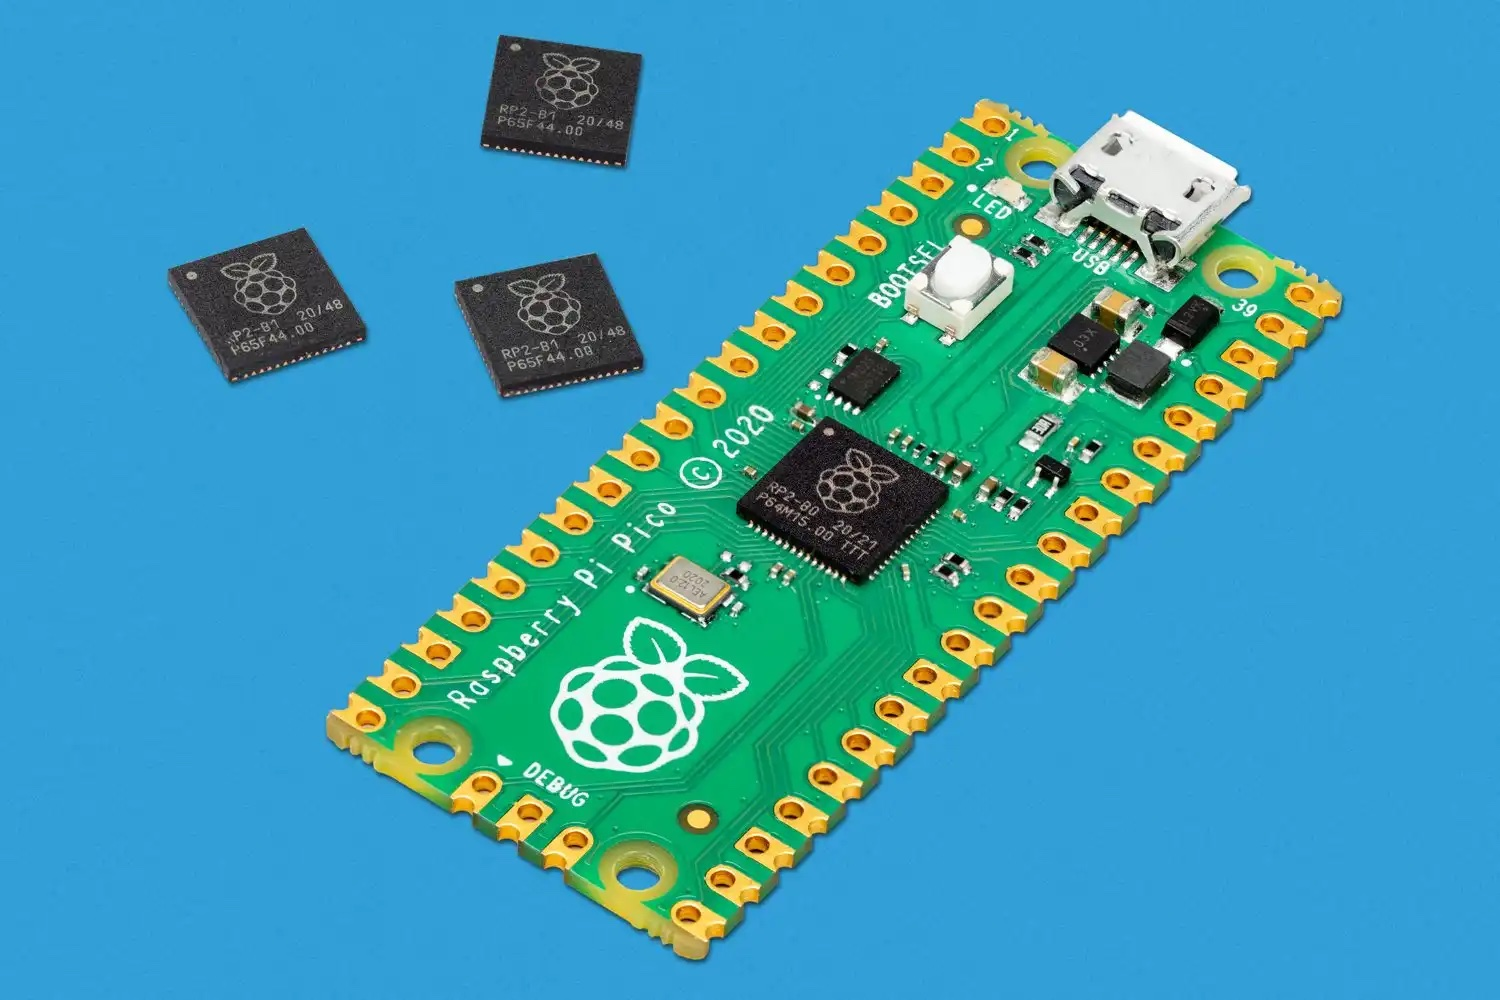
\includegraphics[width=\textwidth]{pico-rp2040}}
	\caption{Stock photo of Raspberry Pi Pico}
	\label{fig:picostock}
\end{figure}

The Raspberry Pi Pico\ref{fig:picostock} is a compact MCU development platform created by the Raspberry pi foundation, running a dual core ARM Cortex M0 at 133Mhz with a generous 264kB inbuilt RAM and 2MB of SPI flash for the class of MCU\cite{ltdRaspberryPiPico}.

\pagebreak
\section{Ways to access raspberry pi pico flash}

There are a couple of potential ways to be able to access the flash memory on the pico to be able to alter or reflash it as desired.

The most common and usually used method is by holding down the 'bootsel' button when plugging the pi into usb, which disabled the SPI flash chip select line temporarily during boot process and causes the MCU to automatically go into flashing mode whereupon the chip presents a virtual fat drive as a mass storage device to the USB host allowing an image to be dragged on and flashed.

This method could be used to run a RAM resident program via specific UF2 loading addresses which could be used to examine the flash memory and run an automatic recovery of a filesystem from micropython without affecting the primary flashed application.

But this method is cumbersome, as it cannot be fully automated due to the requirement of BOOTSEL to enable it whilst plugging in. there is partially viable way to enter recovery mode without pressing BOOTSEL via USB connection using a PICOTOOL binary that can make negotiate a pico running firmwares based on standard USB stack to reboot into recovery mode, but this is inflexible and would not help recovering an application that immiedietly disables USB automatically at boot which is one of the primary requirements of the project.

The other principle method of being able to arbitrarily access flash memory on pico is via the ARM SWD debug interface using the board accessible debug pads intended for direct programming and onchip debugging.

The SWD interface  is always available regardless of firmware setup, and allows full control of the chip thus making it possible to fully automate. The principle disadvantage of this approach is the less convenient physical access to the interface compared to connecting to a USB host.
\pagebreak
\section{SWD interface}
The ARM SWD interface is an ARM microdevices created standard for all arm Cortex CPU's using two wires for clock and signal, that allows bidirectional communication over a single signal wire and a variable host controlled signal speed.

Communication is etablished with a reset sequence, that will always reset the debug units communication to a known start point so that connection can be etablished regardless of current state.

ARM MCU's can also support JTAG protocol debugging, using the same pins as SWD, for chips supporting both, a handshake to establish the protocol being used is needed. But as the pico is an SWD only MCU, this part of the connection protocol is not needed.

Each CPU core has it's own debug unit, along with a third 'reset' unit that can be used to reset the whole MCU

SWD  control allows commanding a debug unit in the MCU, which can read and write memory, control execution. set breakpoints and other debug aiding measures.

SWD itself cannot directly access the flash memory on the pico, to do this the MCU has to be instructed via memory access and process control to perform the accesses required.

This can be done two different ways, direct instructions to perform requires actions can be written into memory
bofore
\pagebreak
\section{UF2 file format}
UF2 is a file format created by Microsoft with the intention of having a simple universal file format for device firmware image updates, that is very easy to support with a minimal loader to manage the flashing on target device, including frequently via a USB mass storage supporting bootloader that presents a virtual file system to the operating system via standard USB mass storage protocol, so that special hardware and software is not needed for firmware updates.


A Uf2 file is made up of 512byte blocks, each of which has a header specifying the blocks address in rom, a family code to indicate what device the image is meant for, crc check values, current and total block count. This is enough information for flashing software to know where to put each part of image as received, and keep track of progress in order to know full image has been received without an explicit end of transfer, which is key to being able to flash images via USB mass storage filesystem write.

The format was choses by the pi foundation as the native image format for the pico due to this simplicity of use, and the pico recovery bootloader presents a usb mass storage virtual FAT file system from it's ROM stored 16kB alongside USB stack and ROM callable routines for functionality including SPI flashrom writing.

The inbuilt bootloader uses the target address of the image to signify whether to load the data into ram for immiediete execution, or to flash and execute from SPI.

\pagebreak
\section{USB Virtual File system}
Standalone SWD control is enough to be able to recover a file system, but in order to fully setup a pico from scratch a flash image to program is needed. This image could be included into the program as a binary include, but this makes updating cumbersome requiring reasemblin and uploaioading a new full binary image to the host pico.

This is typically achieved by setting the pico into bootsel recovery mode and flashing the new combined uf2 image on.

It was figured that a more convenient alternative would be for the device to manage it's own images, which also allows device to signal what firmware is installed to the user via filename.

The project has to support pico original and w editions, so two firmwares need to be stored.

The UF2 format was created for simplicity of flashing to hardware via a bootloader, and is quite wasteful internally, each 256B block of target flash uses a full 512B in the file to make addressing simple, which leads the file to be nearly half empty due to header data for the 256B blocks only occupying a small portion of the remaining 256B.

This header data is mostly static, barring changing addressing data, thus it is possible to generate this data using only a list of addresses per block. This allows the possibility to generate a custom storage format to save storage and allow a standard 2MB pico enough storage to save flash images for typical use cases for both models.

All the UF2 header data barring addresses can be calculated at run time, so only the addresses for each flash block are required to be stored in a header, empty flash does not waste image space, nor non payload areas of the original uf2 image, thus virtually

\pagebreak





